
%For each cluster, the control time at each position in the observed
%area, $T(x,y)$, is calculated with a Monte Carlo simulation. We
%simulate SN~Ia light curves at the cluster redshift at various times
%during the survey, and determine the probability (using the detection
%efficiencies from Fig.~\ref{fig:eff}) that each simulated SN would be
%detected and counted in our SN sample.

We simulate SN~Ia light curves with a distribution of shapes, colors
and absolute magnitudes.  We use the (original) {\sc
salt} \citep{guy05a} prescription in which the diversity of SN~Ia
light curves is characterized as a two-parameter family with an
additional intrinsic dispersion in luminosity.  The two parameters are
the linear timescale of the light curve (``stretch'', $s$) and the
$B-V$ color excess, $c$.  For each simulated SN, $s$ and $c$ are
randomly drawn from the distributions shown in Figure~\ref{fig:dists}
(solid lines). The stretch distribution is based on the
observed distribution in passive hosts
(Fig.~\ref{fig:dists}, left panel, grey histogram) in the
first-year Supernova Legacy Survey (SNLS) sample \citep{sullivan06a}.
Similarly, the color distribution is based on the observed color
distribution (Fig.~\ref{fig:dists}, right panel, grey
histogram) in the first-year SNLS sample \citep{astier06a}.  The
absolute magnitude of each simulated SN is set to
\begin{equation}
M_B = -19.31 - \alpha (s-1) + \beta c + I
\end{equation}
where $-19.31$ is the magnitude of an $s=1$, $c=0$ SN~Ia in our
assumed cosmology \citep{astier06a}, $\alpha = 1.24$, $\beta =
2.28$ \citep{kowalski08a}, and $I$ is an added ``intrinsic
dispersion'', randomly drawn from a Gaussian distribution centered at
zero with $\sigma = 0.15$~mag.

%%%%%%%%%%%%%%%%%%%%%%%%%%%%%%%%%%
% PLOT: SIMULATION DISTRIBUTIONS %
%%%%%%%%%%%%%%%%%%%%%%%%%%%%%%%%%%
\begin{figure}[tbhp]

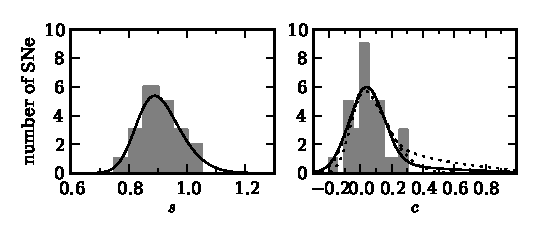
\includegraphics[width=\textwidth]{figures/clrate/dists_cluster.eps}
\caption[Stretch and color distributions of simulated supernovae]
{{\it Left panel:} stretch distribution used for simulated SNe 
(solid line) and the stretch distribution of first-year SNLS
$z<0.75$ SNe in passive hosts \citep{sullivan06a} (grey
histogram). Note that the distribution is not changed significantly
by cutting the sample at $z<0.6$. Therefore we do not expect the
sample to be significantly Malmquist biased. {\it Right panel:} color
distribution of the first-year SNLS $z<0.6$ SNe \citep{astier06a}
(grey histogram) and the color distribution used for simulated
SNe (solid line). The dotted lines show alternative
color distributions used to assess the possible systematic error due
to varying amounts of SNe being affected by dust.\label{fig:dists}}
\end{figure}

We have chosen distributions that represent as accurately as possible
the full distribution of SNe~Ia occurring in reality. However, note
that the control time is not actually very sensitive to the assumed
distributions. This is because, for the majority of cluster redshifts
in the survey, the detection efficiency is close to 100\% during the
time of the survey. Supernovae would thus have to be significantly
less luminous in order to change the detection efficiency
significantly. In the following section \S\ref{sec:ct_sys} we quantify the
effect on the control time arising from varying the assumed SN~Ia
properties and show that they are sub-dominant compared to the Poisson
error in the number of SNe observed. All sources of systematic errors
are also summarized in \S\ref{sec:clrate_results_sys}.

To generate the simulated light curves in the observed bands, we use
the \citet{hsiao07a} SN~Ia spectral time series template. For each
simulated SN, the spectral time series is warped to match the selected
color $c$ and redshifted to the cluster rest-frame. Light curves are
generated in the observed $i_{775}$ and $z_{850}$ filters using
synthetic photometry, and the time axis is scaled according to the
chosen value of $s$.

For each cluster, we calculate $T(x,y)$ in bins of 50 $\times$
50~pixels ($2''.5\ \times\ 2''.5$). In each bin, we simulate 100 SN
light curves at random positions within the bin.  For each simulated
SN light curve, we shift the light curve in time across the entire
range of observations, starting with maximum light occurring 50~days
before the first observation and ending with maximum light occurring
50~days after the last observation. For each step in time we get the
$z_{850}$ and $i_{775}$ magnitude of the SN at every date of
observation. From the sky noise maps, we know the noise at the
position of the simulated SN in every image. Using the curves in
Figure~\ref{fig:eff}, we convert the SN flux-to-noise ratio to the
probability of the SN being detected in each $z_{850}$ exposure. (Each
simulated SN is also assigned a host galaxy surface brightness chosen
from a distribution, in addition to the randomly selected $s$, $c$ and
$I$ parameters; we use the Fig.~\ref{fig:eff} curve that corresponds
to this surface brightness.) At the same time, we calculate the
probability that the SN passes our light curve cuts (using both
$z_{850}$ and $i_{775}$ simulated magnitudes). Multiplying these two
probabilities gives the total probability of the simulated SN being
included in the sample if it peaks at the given date.  Integrating the
probability over time (the entire range of dates) gives the control
time for each simulated SN. We take the average control time of the
100 SNe as the value for the given bin. The resulting control time
map, $T(x,y)$, therefore has a resolution of $2''.5\ \times\
2''.5$. $T(x,y)$ is shown for two example clusters in
Figure~\ref{fig:ctmaps}.

%%%%%%%%%%%%%%%%%%%%%%%%%%%%%%%%%%
% PLOT: CTMAPS                   %
%%%%%%%%%%%%%%%%%%%%%%%%%%%%%%%%%%
\begin{figure}

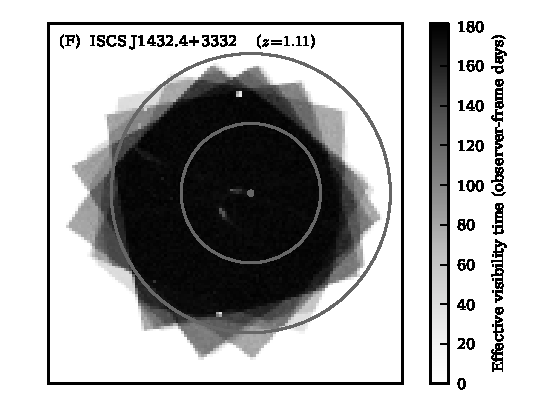
\includegraphics[width=0.5\textwidth]{figures/clrate/ctmap_f.eps}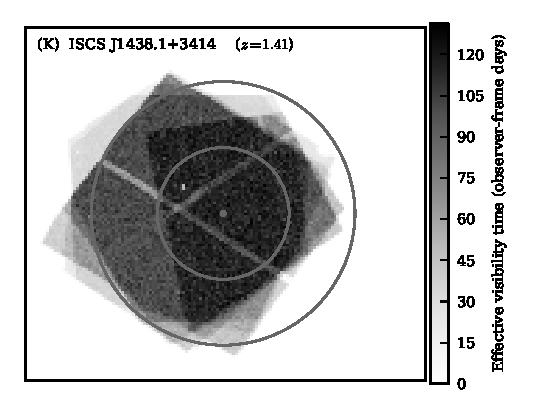
\includegraphics[width=0.5\textwidth]{figures/clrate/ctmap_k.eps}
\caption[Example maps of effective visibility times]
{Example maps of effective visibility time for clusters 
ISCS J1432.4+3332 (F) and ISCS J1438.1+3414 (K).  The dot denotes the
cluster center and the inner and outer circles represent 0.5~Mpc and
1.0~Mpc radius, respectively. The ``noise'' in these maps is due to
the finite number (100) of SNe simulated at each position.  At lower
redshift nearly all simulated SNe are recovered at each position,
whereas at higher redshift a sizable fraction of simulated SNe are
missed, resulting in a higher ``noise'' level.
\label{fig:ctmaps}}
\end{figure}
